\chapter{Desarrollo}\label{sec:des}
\section{Arquitectura de \omnetpp{}}

Tomemos como punto de partida la siguiente definición de módulo simple en C++
(obviando la implementación de los métodos que no son relevantes en este
momento).

\inputminted{c++}{codelistings/txc1.cc}

Luego de compilar de dicho modelo junto al kernel de simulación, el binario
logra crear instancias del módulo \verb!Txc1! (tantas como los archivos NED
indiquen en la descripción de la topología de la red) e invocar a sus métodos.
Nuestro próximo objetivo es entender los mecanismos puestos en juego por
\omnetpp{} para lograr esto. Se exponen a continuación los principales elementos
que contribuyen a entender la solución encontrada.

\subsection{El ciclo de vida de una simulación}

Cuando el usuario ejecuta el binario de una simulación el inicio de la
ejecución ocurre en la función main donde únicamente se llama a
\verb!omnetpp::envir::evMain! con los argumentos recibidos del sistema
operativo. En esta última función se llama a \linebreak
\verb!setupUserInterface!, nuevamente pasando los argumentos de invocación del
programa.

Esta función presenta tres etapas claramente señaladas mediante comentarios en
el código:

\begin{enumerate}
    \item SETUP (preparación): procesamiento de la configuración, instanciación
de una interfaz de usuario (gráfica o de consola).

    \item RUN (ejecución): el entorno creado (qtenv, o cmdenv o tkenv) es
efectivamente puesto a correr. Los tres tipos de ambientes comparten mucho
código y terminan llamando a código común en una clase base para correr la
simulación. Aquí se consumen los eventos (mensajes) que los módulos van
generando y enviando. Si se acaban los eventos o se acaba el tiempo designado
para la simulación, esta finaliza.

    \item SHUTDOWN (finalización): limpieza final, antes de devolver el valor
de retorno de la simulación.
\end{enumerate}

Nos interesa particularmente lo que ocurre en las etapas de SETUP y SHUTDOWN,
por lo que podemos obviar los llamados que ocurren en RUN. La figura~\ref{fig:symlc}
permite entender mejor lo expuesto y dónde estamos poniendo el foco de
atención.

\begin{figure}[h]
\caption{Ciclo de vida de una simulación}
\label{fig:symlc}
\centering
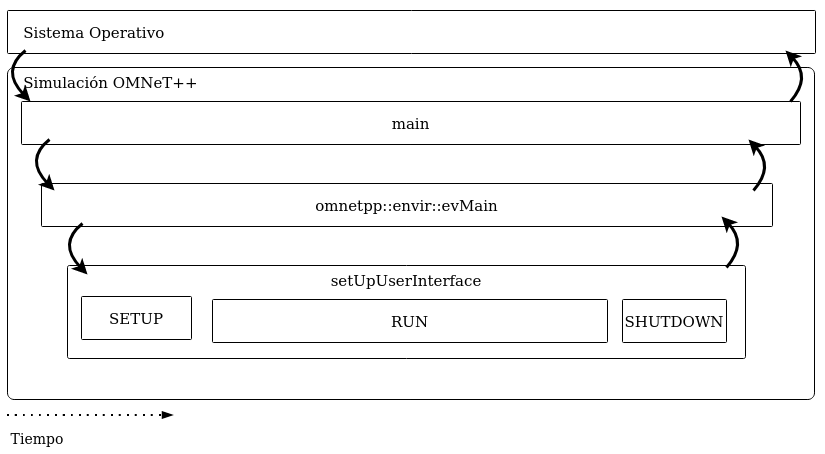
\includegraphics[width=\textwidth]{sym_lifecycle}
\end{figure}
\subsection{Code fragments: ejecución de código genérico}

Existe en \omnetpp{} una clase denominada \verb!CodeFragments!, la cual
analizamos a continuación.

Una instancia de \verb!CodeFragments! se inicializa con dos argumentos:

\begin{enumerate}
    \item un puntero a una función de tipo \verb!void -> void!.
    \item una instancia de un tipo enumerado que representa cuándo debe ser ejecutada tal función:
    \begin{itemize}
        \item \verb!CodeFragments::STARTUP! para designar a las funciones a correr durante la etapa de preparación
        \item \verb!CodeFragments::SHUTDOWN! para designar a las funciones a correr durante la etapa de finalización
    \end{itemize}
\end{enumerate}

A su vez, \verb!CodeFragments! tiene atributos de clase (\verb!head! y
\verb!next!) que sirven para implementar una lista enlazada global. Cada vez
que se inicializa una variable de tipo \verb!CodeFragments! esta se coloca como
cabeza de la lista y almacena un puntero al siguiente elemento (la última de
las instancias que se crearon antes que ella), es decir que se inserta por
delante y hace crecer la lista.  Esta estructura de datos se conoce como
``stack'' o pila.

Existe también la función de clase \verb!CodeFragments::executeAll!, que toma
un tipo (ya sea \verb!CodeFragments::STARTUP! o \verb!CodeFragments::SHUTDOWN!)
y recorre toda la lista, ejecutando las funciones de aquellos
\verb!CodeFragments! que tienen el tipo especificado.

Cerca del inicio de la simulación, durante la estapa de STARTUP se ejecuta

\begin{minted}[linenos=false]{c++}
CodeFragments::executeAll(CodeFragments::STARTUP);
\end{minted}

mientras que cerca del final de la simulación, durante la etapa de SHUTDOWN, se ejecuta:

\begin{minted}[linenos=false]{c++}
CodeFragments::executeAll(CodeFragments::SHUTDOWN);
\end{minted}

Este es un dato muy importante, ya que nos proveerá un mecanismo para manejar el ciclo de vida del intérprete de Python embebido,
lo cual será abordado en la sección~\ref{subsec:interpreterlifecycle}

\subsection{El registro global de clases}

A la hora de construir la red para lanzar la simulación, \omnetpp{} va creando
recursivamente los módulos y sus submódulos a partir de su nombre (proveniente
de los archivos NED). Es necesario pasar de un simple string como \verb!"Txc1"!
o \verb!"Tictoc"! a un objeto de la clase apropiada.

Para tal fin, \omnetpp{} cuenta con la clase \verb!cRegistrationList!, la cual
implementa un mapeo de tipo \verb!std::string -> omnetpp::cOwnedObject*!. Para
lograr que tal mapeo sea único y que sea accesible desde cualquier punto del
programa, la clase \verb!cGlobalRegistrationList! implementa una variación del
patrón de diseño conocido como ``singleton''. En efecto, no hay una única
instancia de \verb!cRegistrationList!, si no que hay una especializada para
cada tipo de objeto. En particular, existe una de estas
\verb!cGlobalRegistrationLists! llamada \verb!classes! donde se mapea de
nombres de tipos (por ej, \verb!"Txc1"!, \verb!"Tictoc"!, etc.) a instancias de
\verb!omnetpp::cObjectFactory!.

¿Qué es un \verb!cObjectFactory!? Cada instancia de \verb!cObjectFactory! sabe
cómo crear objetos de un tipo determinado. Almacena una función de creación,
una función de casteo y una descripción en forma de string.

Poniendo todas estas piezas juntas, lo que \omnetpp{} hace para obtener una
instancia de un módulo, en la etapa de construcción de la red (se omite el
manejo de errores):

\begin{itemize}
    \item llama al método de clase \verb!cObjectFactory::createOne(className)!

    \item el método de clase busca en el \verb!cGlobalRegistrationList! llamado
\verb!classes! al \verb!cObjectFactory! apropiado para tal nombre de clase

    \item una vez identificado el \verb!cObjectFactory! adecuado, se llama a la
función de creación que este contiene.

\end{itemize}

Todo este andamiaje es transparente para el usuario. Su única responsabilidad
es definir un módulo que herede de \verb!cSimpleModule!, y presentarlo al
sistema mediante \verb!Define_Module!. Todos estos detalles sobre cómo hace
\omnetpp{} para instanciar su clase están ocultos.

Es importante descubrir, entonces, quién provee el \verb!cObjectFactory! que
sabe construir y castear instancias del módulo definido por el usuario, y
además, quién registra ese \verb!cObjectFactory! en la instancia global de
\verb!cGlobalRegistrationList! llamada \verb!classes!.

\subsection{El macro \texttt{Define\_Module}}

Luego de la definición de la clase \verb!Txc1!, para su uso en una simulación
es mandatorio escribir \verb!Define_Module(Txc1);!. Sin esta instrucción,
\omnetpp{} simplemente no toma conocimiento del módulo agregado por el usuario.

\verb!Define_Module! parece a simple vista una función, sin embargo es un
macro, cuya definición luce así:

\inputminted{c++}{codelistings/define_module_1.cc}

Esta definición involucra al macro \verb!__REGISTER_CLASS!, que a su vez está
construido sobre otro macro:

\inputminted{c++}{codelistings/define_module_2.cc}

Expandiendo recursivamente todos los macros involucrados (por ejemplo,
utilizando la opción \verb!-E! del compilador) y formateando el espaciado para
mejorar la legibilidad se logra ver que \verb!Define_Module(Txc1);! termina
convirtiéndose en:

\inputminted{c++}{codelistings/define_module_3.cc}

Analicemos un poco el resultado.

\verb!static omnetpp::cObject *__factoryfunc_13()!: define una ``factory
function'', encargada de la creación de nuevas instancias de \verb!Txc1!.

\verb!static void *__castfunc_13(omnetpp::cObject *obj)!: define una función de
casteo, que a partir de un puntero a una instancia de \verb!omnetpp::cObject!
devuelve el resultado de reinterpretar ese puntero como un puntero a instancia
de \verb!Txc1!.

\verb!void __onstartup_func_13()!: define una función que registra ante \omnetpp{}
la existencia de un nuevo tipo de módulo simple llamado \verb!Txc1!, junto con
las funciones de creación y casteo definidas ad hoc.

Se hace notar que los nombres incluyen el número ``13'' porque en el archivo
original, \verb!Define_Module(Txc1)!; estaba escrito en la línea 13. Con esto
se busca diferenciar funciones en el potencial caso de tener diversos usos del
macro \verb!Define_Module! en el mismo archivo. Efectivamente encontramos que,
de ejecutarse la función \verb!__onstartup_func_13!, \omnetpp{} pasaría a tener
conocimiento de un módulo llamado \verb!"Txc1"! y contaría con un mecanismo
para crear instancias del mismo.

Notar que hasta el momento se trata de definiciones de funciones, pero ninguna
de ellas ha sido invocada. Lo que sigue es diferente:

\inputminted{c++}{codelistings/define_module_4.cc}

Esto es una declaración e inicialización de una variable estática. Como
tal, su inicialización ocurre al comenzar la ejecución del programa. Es decir
que antes de que la función \verb!main! sea invocada, esta llamada a
constructor ya se ejecutó y por lo tanto la instancia de \verb!CodeFragments!
que se acaba de crear ya se encuentra formando parte de la lista global de
\verb!CodeFragments!. Por lo tanto, el resultado final de la instanciación de
esta variable es la colocación de \verb!__onstartup_func_13!  de para ser
ejecutada durante la etapa de STARTUP de la función \verb!setupUserInterface!.
Más aún, cuando esa función se ejecute, el resultado es que se registra ante
\omnetpp{} un tipo de módulo simple nuevo (\verb!Txc1!) así como las funciones
necesarias para su creación y casteo. Esto permitirá a \omnetpp{} crear y
manipular instancias de \verb!Txc1!  cuando sea necesario (según lo dicten los
archivos de descripción de la topología de la red).

En resumidas palabras, el macro \verb!Define_Module(T)!  (donde \verb!T! es la
clase definida por el usuario) sirve para:

\begin{enumerate}
    \item definir una función (F1) de creación de objetos del tipo \verb!T!

    \item definir una función (F2) de casteo a objetos del tipo \verb!T!

    \item definir una función (F3) que registra ante \omnetpp{} el tipo
\verb!T! junto con las funciones F1 y F2.

    \item definir una variable de tipo \verb!CodeFragments! que al ser estática
se inicializa antes de llamar a la función principal del programa. Esto último
garantiza que F3 se ejecuta durante la etapa de STARTUP de
\verb!setupUserInterface! y, como consecuencia, cuando llega el momento de
instanciar a la clase \verb!Txc1!, \omnetpp{} ya puede hacerlo.

\end{enumerate}

\section{Registrando módulos Python}

Luego de conocer el ciclo de vida de la simulación en \omnetpp{}, los mecanismos
que se activan a la hora de declarar un módulo escrito por el usuario (puestos
en juego por el macro \verb!Define_Module!) así como el andamiaje provisto por
\verb!CodeFragments! y las llamadas

\begin{minted}[linenos=false]{c++}
CodeFragments::executeAll(CodeFragments::STARTUP);

CodeFragments::executeAll(CodeFragments::SHUTDOWN);
\end{minted}

\noindent que realiza la función \verb!setupUserInterface!, se empieza a definir una
estrategia para la implementación de módulos directamente en Python.

En una primera etapa, buscamos definir una serie de funciones y definiciones
que hagan en su conjunto lo mismo que el macro anteriormente estudiado.
Convertir todo ese código en un macro lo más sencillo posible sería bueno (para
la comodidad del usuario), pero por el momento se posterga.

Buscamos:

\begin{itemize}
    \item Una función que al ser invocada (sin argumentos) devuelva un puntero
a una instancia de \verb!PySimpleModule! convertido a puntero a instancia de
\verb!cModule!.

    \item Una función de casteo a objetos del tipo \verb!PySimpleModule!.

    \item Una función que sea registrada (como un \verb!CodeFragment!) para ser
ejecutada durante la etapa de SETUP de \verb!setupUserInterface! para registrar
este nuevo tipo ante \omnetpp{}. 

\end{itemize}

A su vez, es necesario inyectar en el ciclo de vida de \omnetpp{} la
inicialización y finalización del intérprete de Python.

Por último, es necesario que el usuario pueda especificar clases en Python
heredando de una clase base que sea la versión Python de \verb!cSimpleModule!,
de forma de poder realizar los casteos a los tipos de C++ que espera \omnetpp{}.

\subsection{\texttt{PySimpleModule}: heredando \texttt{cSimpleModule} en Python}

Comenzamos a trabajar en extender el intérprete de Python con las clases de\linebreak
\omnetpp{}. En una primera etapa se trabajó en exponer sólo aquello que era
estrictamente necesario para lograr la implementación de la primera parte del
tutorial tictoc: las clases \verb!cSimpleModule! con los métodos
\verb!getName! y \verb!send!, y la clase \verb!cMessage!.

También fue en esta etapa en que se trabajó efectivamente con pybind11 por lo
que fue también un momento de exploración de esta herramienta (cuya elección
probó ser acertada).

Se incluye aquí la primera versión exitosa del código que se utilizó para
exponer estas clases, con el objetivo de que el lector tenga noción del tipo de
trabajo que se estaba realizando.

\inputminted{c++}{codelistings/binding.cc}

Luego de la compilación de ese archivo en C++ se obtiene un módulo en Python
que expone las clases \verb!cSimpleModule!, \verb!cMessage!, así como algunos
de sus métodos. Es decir, estamos en condiciones de escribir en Python algo
como:

\inputminted{Python}{codelistings/binding_usage.py}

Como puede verse en el siguiente uso interactivo, estas clases no son útiles
fuera del contexto de una simulación:

\begin{minted}[linenos=false]{text}
# python3
>>> from pyopp import cSimpleModule, cMessage
>>> sm = cSimpleModule()
>>> sm.handleMessage(cMessage('hello'))
<!> Error during startup/shutdown: Global simtime_t variable found, with value 0. Global simtime_t variables are forbidden, because scale exponent is not yet known at the time they are initialized. Please use double or const_simtime_t instead. Aborting.
\end{minted}

No obstante, ya contamos con la extensión necesaria para que el código escrito
por el usuario herede en Python de la clase \verb!cSimpleModule! (escrita en
C++). A continuación exploramos cómo integrar estas clases en una simulación.

\subsection{Creación de módulos definidos en Python desde C++}

Para lograr que \omnetpp{} sepa cómo instanciar esta clase definida en Python el
paso siguiente fue definir la factory function necesaria. Una primera versión
de la misma luce así:

\inputminted{c++}{codelistings/factory_function.cc}

Esta factory function es esencialmente lo que buscamos, excepto por dos
motivos. El primero de ellos es la conversión intermedia a
\verb!cSimpleModule!, necesaria porque C++ y pybind11 no conocen la relación
entre nuestra clase definida en Python y \verb!cObject!. En una futura versión,
en la que el módulo expuesto a Python incluye toda la jerarquía de clases base
de \verb!cSimpleModule! (la cual tiene a \verb!cObject! en la raíz), este paso
intermedio puede eliminarse.

El segundo motivo, mucho más complejo y difícil de resolver es que al terminar
el scope de la función, el objeto Python que acaba de ser creado es eliminado
de la memoria por el intérprete de Python. Para entender por qué esto es así,
necesitamos hablar de cómo Python maneja la memoria y el ciclo de vida de sus
variables.

Recordemos que en C++, los principales lugares donde las variables pueden
existir son:

\begin{description}
    \item[el stack (manejo automático):] variables declaradas sin manejo
explícito de la memoria y son liberadas tan pronto como salen de scope (el
bloque de código que las contiene). Para alojar una variable en el stack, el
compilador debe conocer su tamaño. Además, el espacio del stack es bastante
limitado.

    \item[el heap (manejo manual):] una fuente mucho mayor de memoria,
administrada por el sistema operativo. Las variables cuya memoria se pide y se
devuelve explícitamente tienen un ciclo de vida independiente del stack y el
compilador no necesita conocer su tamaño.
\end{description}

Naturalmente, Python aloja todos los objetos creados por el usuario en el heap.
A su vez, con el propósito de liberar la memoria de aquellas variables que ya
no se utilizan, cada objeto Python contiene información de cuántas referencias
hay a él en un programa (variables que sirven para alcanzarlo). Digamos que en
el ejemplo:

\begin{minted}[linenos=false]{Python}
a = 'hola'
b = [a]
\end{minted}

El objeto apuntado por la variable a es referenciado en dos lugares (por la
variable \verb!a! y como primer elemento de la lista \verb!b!). Tan pronto como
hacemos:

\begin{minted}[linenos=false]{Python}
b[0] = 'chau'
a = 1
\end{minted}

\noindent el objeto de tipo string \verb!'hola'! que el intérprete de Python
alojó en memoria dinámica ya no es necesario, puesto que no existen referencias
a él. No hay manera de que el programa vuelva a utilizarlo. Es susceptible de
ser eliminado para devolver la memoria al sistema operativo.

El algoritmo que el intérprete utiliza para reconocer este tipo de situaciones
(cuándo es momento de destruir un objeto y devolver su memoria) se conoce como
``reference counting''. Básicamente consiste en incrementar la cuenta cada vez
que se crea una referencia y decrementarla cuando se destruye o sobreescribe
una referencia. Cuando la cuenta se vuelve cero el objeto se puede borrar. No
existen garantías de que el objeto sea borrado inmediatamente, pero el garbage
collector puede hacerlo a partir de ese momento.

Con esta información, no es difícil ver que existe una única referencia al
objeto creado en la línea

\begin{minted}[linenos=false]{c++}
 py::object obj = py_module.attr("PyTxc1")();
\end{minted}

Tan pronto como la variable \verb!obj! (que apunta a un objeto Python en el
heap pero está en el stack) sale de scope y es destruida, el intérprete
reconoce que ya no hay variables apuntando a dicho objeto (desconoce el casteo
a \verb!cSimpleModule*! o \verb!cObject*!) y lo borra (devuelve la memoria al
sistema operativo). Por su lado, el programa \omnetpp{} continúa utilizando la
referencia \verb!ret! que ahora apunta a memoria que es del sistema operativo.
Tan pronto como trate de dereferenciarla, tendremos un \verb!Segmentation Fault!
y el sistema operativo terminará el programa.

La solución implementada fue sencillamente incrementar el contador de
referencias de forma manual antes de que termine la función. 

\begin{minted}[linenos=false]{c++}
    // Instanciamos la clase, obteniendo un py::object
    py::object obj = py_module.attr("PyTxc1")();
    obj.inc_ref();
\end{minted}

Esto evita que el intérprete devuelva la memoria al sistema operativo y permite
que \omnetpp{} utilice la referencia devuelta por la función sin incurrir en un
comportamiento ilegal.

Sin embargo, esto genera un problema simétrico: ahora el objeto Python no será
liberado nunca. Incluso cuando C++ destruya la instancia de cObject que le
devolvimos, el objeto Python seguirá existiendo, ya sin referencias asociadas a
él. Para evitar esto se procedió a decrementar el contador de referencias en el
destructor de la clase base que expusimos a Python:

\begin{minted}[linenos=false]{c++}
~PycSimpleModule() {
    py::object obj = py::cast(this);
    obj.dec_ref();
} 
\end{minted}

Irónicamente, el código del módulo generado por pybind11 se da cuenta de el
objeto C++ que se está borrando es un wrapper a un objeto Python. Al llegar a
cero la cuenta de referencias de dicho objeto, el wrapper debe ser eliminado
también. Este sería el comportamiento correcto si el programa principal fuera
Python y se están invocando librerías escritas en C++. En nuestro caso, es un
``double delete'' o un segundo intento de borrar el objeto.

Borrar un objeto que ya ha sido borrado y cuya memoria ya ha sido devuelta al
sistema operativo es lo mismo que intentar borrar (liberar) una porción de
memoria que ya no nos pertenece. Es otra falta que se penaliza con la
terminación inmediata del programa.

Afortunadamente para nosotros, pybind11 provee un mecanismo para generar código
que no invoca al destructor del objeto C++ una vez que el objeto Python es
liberado.

En resumidas cuentas, el problema se solucionó aplicando las siguientes reglas:

\begin{enumerate}
    \item La cuenta de referencias del objeto Python creado en la factory
function que será llamada por \omnetpp{} debe ser incrementada manualmente,
para evitar que el intérprete decida liberar su memoria tan pronto como la
función retorna.

    \item Cuando \omnetpp{} libera el objeto C++ que en realidad es el wrapper
de un objeto Python, la cuenta de referencias del objeto Python debe ser
decrementada para permitir que su memoria sea liberada.

    \item Pybind11 no debe eliminar el objeto C++ que envuelve al objeto Python
cuando este último sea liberado.
\end{enumerate}

Este problema del ciclo de vida de los objetos volverá a aparecer más adelante
con los mensajes que se crean en un módulo con destino a otro módulo. El
escenario es ligeramente diferente y la solución encontrada, también. Se lo
describe más adelante.

\subsection{La función de casteo}

El único uso que se hace de la función de casteo es en el método de
\verb!cObjectFactory!

\begin{minted}[linenos=false]{c++}
/**
* Returns true if the given object can be cast
* (via dynamic_cast) to the class represented by
* this factory object, and false otherwise.
*/
virtual bool isInstance(cObject *obj) const  {
    return castFunc(obj)!=nullptr;
}
\end{minted}

el cual utiliza la posibilidad o imposibilidad de castear el objeto a la clase
declarada como signo de que el objeto en cuestión es o no es instancia de la
misma. Nuestra primera versión de la función de casteo es:

\begin{minted}[linenos=false]{c++}
static void *F2(omnetpp::cObject *obj) {
    return (void*)dynamic_cast<PycSimpleModule*>(obj);
}
\end{minted}

Notar que esta función devolverá \verb!true! para cualquier objeto que haya
sido implementado en Python heredando de \verb!cSimpleModule!. No sirve para
identificar las clases derivadas en Python.

No obstante, no seguimos trabajando en una función de casteo más elaborada por
considerarlo innecesario. Inspeccionando el código de \omnetpp{} se puede
constatar que la función \verb!isInstance! se llama sólamente para validar el
tipo del tercer argumento de la función cComponent::emit. Dicho tercer
argumento es de tipo \verb!cObject*! y tiene como valor por defecto nullptr. No
encontramos ejemplo de su uso en la documentación ni en ninguno de los samples.

\subsection{Ciclo de vida del intérprete}\label{subsec:interpreterlifecycle}

Resta proveer un mecanismo que asegure que un intérprete de Python está vivo
durante el tiempo que esto es estrictamente necesario. Es decir, desde antes de
la primera instanciación de nuestros módulos hasta después de la destrucción
del último de ellos.

Se logró instanciando un \verb!pybind11::scoped_interpreter! (sólo uno) que se
mantiene vivo a lo largo de toda la aplicación.

\begin{minted}[linenos=false]{c++}
class InterpreterManager {
  private:
    static void* interpreter;
  public:
    static void ensureInterpreter();
};
\end{minted}

La implementación de \verb!ensureInterpreter! simplemente valida que
\verb!interpreter! sea un puntero nulo (lo cual sirve para identificar la
primera vez que llaman a la función).

Una solución alternativa podría ser agregar la línea

\begin{minted}[linenos=false]{c++}
pybind11::scoped_interpreter guard{};
\end{minted}

\noindent al comienzo de la función \verb!main! de \omnetpp{}.  Esta solución
no nos seduce porque queremos dejar el código original de \omnetpp{} lo más
intacto posible.

\subsection{Juntando todas las piezas}

En resumidas cuentas, este es el código que hay que escribir para que \omnetpp{}
levante nuestra implementación del módulo desde un archivo Python:

\inputminted{c++}{codelistings/omnetpy.cc}

\subsection{El macro \texttt{Define\_Python\_Module}}

No es difícil ver que el código anterior, necesario para registrar módulos
Python, es esencialmente siempre el mismo, con excepción del nombre del módulo
así como el nombre del archivo donde este vive.

Con el objetivo de facilitar el registro de módulos hechos en Python, en
paralelo al macro \verb!Define_Module!, se creó un macro
\verb!Define_Python_Module!. En esencia, esto es todo el código C++ que un
usuario debe escribir para lograr el mismo resultado que en el ejemplo
anterior:

\inputminted{c++}{codelistings/pytxc.cc}

Donde la clase \verb!PyTxc! está definida en el archivo \verb!txc.py!, y se
asume que el mismo puede ser importado sin errores (esto es, \verb!import txc!
no produce errores).

\section{Generalización}

Con el desarrollo presentado hasta aquí en esta sección, queda logrado el
objetivo de hacer que \omnetpp{} instancie clases definidas en Python y las acepte
como implementación de módulos de una simulación. El trabajo hecho para
extender el intérprete (exponer las clases de C++ como módulos Python) incluyó
lo mínimo necesario para poder correr las versiones más simples del tutorial
oficial tictoc. 

A continuación, se prosiguió escribiendo en Python el resto del tutorial
tictoc. Este tutorial tiene unas 17 simulaciones progresivamente más complejas
(aún sobre la idea de dos módulos que se intercambian el mismo mensaje).

En cada iteración se fueron agregando nuevas funcionalidades que debían ser
expuestas a Python (es decir, los bindings debían ser extendidos para incluir
más código de \omnetpp{} y hacerlo accesible desde Python).

Algunas nuevas funcionalidades se resolvieron simplemente agregando una
definición en el módulo de los bindings, otras presentaron desafíos mayores
(borrado de mensajes, logging).

Poco a poco, los principales features de \omnetpp{} fueron soportados en un módulo
Python:

\begin{itemize}
    \item recolección de parámetros desde los archivos de configuración
    \item logging (el macro \verb!EV!)
    \item emisión de señales
    \item manipulación de gráficos en la UI
    \item \verb!WATCH!
\end{itemize}

Luego de concluir las simulaciones propuestas en el tutorial tictoc se comenzó
a implementar en Python las simulaciones provistas en el directorio samples
(contiene diversos ejemplos diseñados para mostrar el potencial de la
herramienta). Esto permitió seguir ampliando la superficie de código expuesta a
Python.

Asimismo, se encontraron algunas limitaciones para las cuales no se encontró
una solución, las cuales se encuentran detalladas en la
sección~\ref{subsec:lim}.

\subsection{Mas allá de \texttt{cSimpleModule} y \texttt{cMessage}}

Las clases de \omnetpp{} más elementales para una simulación son las dos
mencionadas en el título. \verb!cSimpleModule! es la clase que el usuario debe
extender para construir sus agentes de simulación, y \verb!cMessage! es la clase
utilizada para producir eventos que empujen el desarrollo de la simulación.
Estas son las únicas clases empleadas en las primeras versiones del tutorial
tictoc y, por lo tanto, fueron las primeras que se expusieron a Python en una
primera etapa exploratoria. Una vez que se vio que el enfoque adoptado fue
exitoso, se procedió a exponer a Python una mayor superficie de la librería de
simulación de \omnetpp{}. Qué exponer y en qué orden fue organizado en torno a
desarrollar en Python los mismos ejemplos que se proveen en el directorio
\verb!samples! del proyecto original. Esto permitió también ir comparando los
resultados de las simulaciones hechas en C++ con las simulaciones hechas en
Python.

Este proceso de migración paulatina de los ejemplos (samples) a Python permitió
enriquecer notablemente el rango de posibilidades de la librería \verb!pyopp!
(el binding expuesto a Python), añadiendo funcionalidad esencial para un
simulador de eventos discretos:

\begin{itemize}
    \item recolección de métricas (clases \verb!cStatistic!, \verb!cStdDev!,
    \verb!cAbstractHistogram!, \linebreak \verb!cHistogram!,
    \verb!cHistogramStrategy!, \verb!cOutVector!),

    \item acceso al tiempo de simulación (clase \verb!cSimTime!),

    \item manipulación de la representación gráfica de la simulación (clases
    \verb!cCanvas!, \linebreak \verb!cDisplayString!)

    \item parametrización de experimentos (clase \verb!cPar!)

    \item cambios dinámicos en la organización del modelo (clase
\verb!cTopology!, \verb!cGate!, \verb!cChannel!, \verb!cDataRateChannel!)
\end{itemize}

\subsection{El macro \texttt{EV}}\label{subsec:ev}

Existe en \omnetpp{} algo que luce como un objeto (aunque es en realidad un macro)
que sirve para generar mensajes desde el código. Estos mensajes se verán en la
interfaz gráfica de la simulación en un tablero especial destinado a tal fin.

Por ejemplo, el siguiente código (samples/aloha/Host.cc):

\begin{minted}[linenos=false]{c++}
EV << "generating packet " << pkname << endl;
\end{minted}

\noindent produce este efecto en la simulación (ver sección inferior derecha de
la fig.~\ref{fig:aloha_EV}).

\begin{figure}[h]
\caption{Uso de \texttt{EV} en simulación aloha}
\label{fig:aloha_EV}
\centering
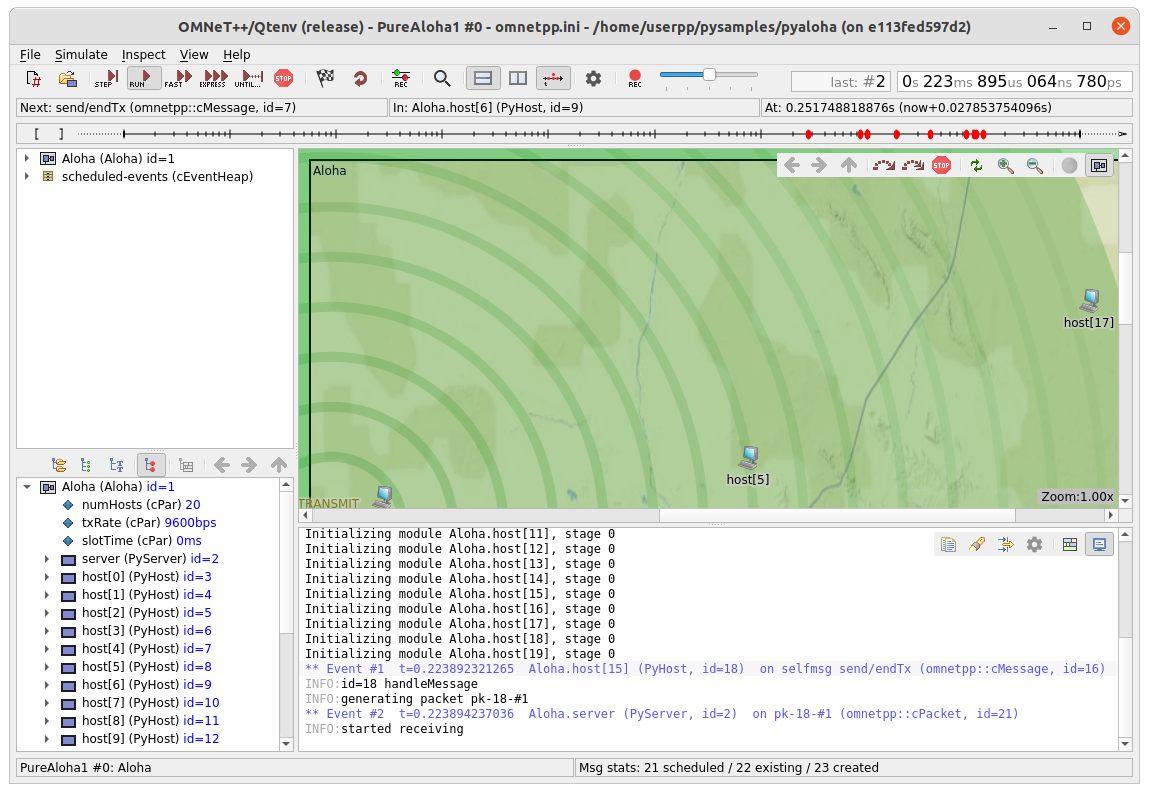
\includegraphics[width=\textwidth]{aloha_EV}
\end{figure}

Este macro hace mucho más que simplemente aceptar una cadena de caracteres:
captura el contexto de quién envía el mensaje, de forma que en la interfaz
gráfica se pueden filtrar mensajes por su origen, como se aprecia en la
figura~\ref{fig:aloha_filter}

\begin{figure}[h]
\caption{Filtrado de mensajes}
\label{fig:aloha_filter}
\centering
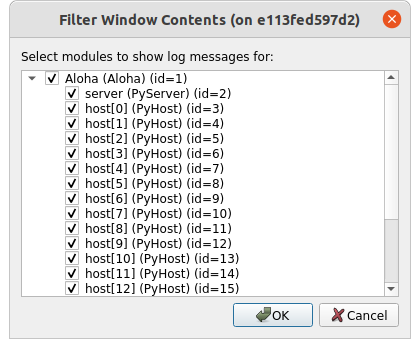
\includegraphics[width=6cm]{aloha_filter}
\end{figure}

% TODO imagen

A su vez, \verb!EV! es un alias de \verb!EV_INFO!, y existen \verb!EV_WARN!,
\verb!EV_DEBUG!, \verb!EV_DETAIL!, etc.

Al portar esta funcionalidad a Python se buscó que la sintaxis fuera lo más
similar posible:

\begin{minted}[linenos=false]{Python}
from pyopp import EV
...
pkname = "pk-%d-#%d" % (self.getId(), self.pkCounter)
EV << "generating packet " << pkname << '\n'
\end{minted}

Este objeto EV se hace cargo de investigar el stack de Python para descubrir
quién emitió el mensaje y crear así un objeto usando la verdadera API de
\omnetpp{} (oculta al usuario de \verb!omnetpy!, para simplificar).

\subsection{\texttt{WATCH}: inspección del estado desde la GUI}

\verb!WATCH! es otra herramienta de \omnetpp{} que apunta a facilitar la
trazabilidad de las simulaciones. Se trata de un mecanismo que permite declarar
interés en observar permanentemente el estado de cierta variable o cierto
atributo de un módulo. Suponiendo que existe la variable \verb!counter!, su uso
desde el código sería sencillamente:

\begin{minted}[linenos=false]{c++}
WATCH(counter)
\end{minted}

Para acceder a la información de la variable en tiempo real desde el entorno
gráfico de la simulación, podemos seleccionar \ui{Inspect $\rightarrow$ Find /
Inspect objects}, y utilizar los filtros disponibles hasta dar con lo que nos
interesa, como se muestra en la figura~\ref{fig:tictoc_inspect}.

\begin{figure}[h]
\caption{Inspección de objetos}
\label{fig:tictoc_inspect}
\centering
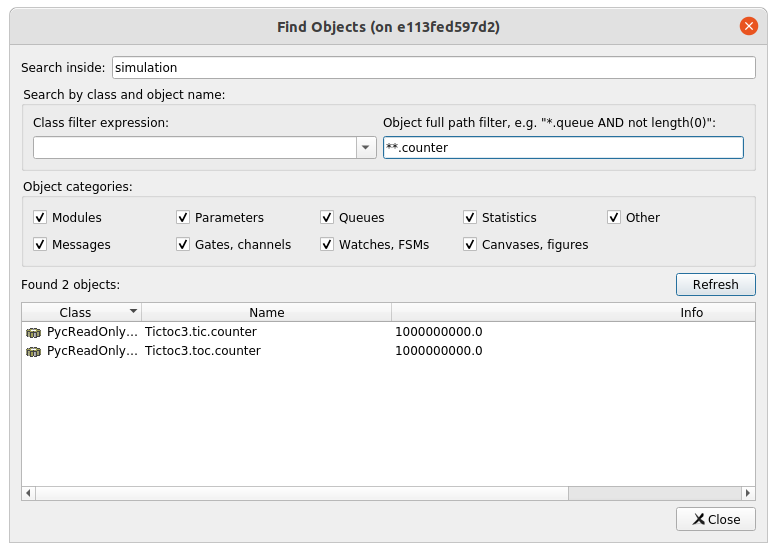
\includegraphics[width=10cm]{tictoc_inspect}
\end{figure}

Esta funcionalidad también se expuso a Python, con la sola diferencia de que
hay que pasar un string con el nombre de la variable que queremos monitorear:

\begin{minted}[linenos=false]{Python}
WATCH('counter')
\end{minted}

\subsection{Recolección de estadísticas}

Los datos generados durante una simulación (los sucesivos tiempos de arribo, de
demora, paquetes perdidos, paquetes corruptos, etc.) pueden ser recolectados:

\begin{itemize}
    \item como pares de (tiempo, valor) como una serie temporal
    \item como valores atemporales, utilizados para calcular media, varianza,
etc.
\end{itemize}

Estos datos son recogidos ya sea en cada invocación del método
\verb!handleMessage!, o bien en el método \verb!finish!, el cual se suele
aprovechar para escribir los datos a un archivo en disco.

Los datos generados son escritos en archivos en el subdirectorio results dentro
del directorio de la simulación, y pueden posteriormente ser analizados
utilizando el IDE (entorno de desarrollo integrado).

Las clases necesarias para esta actividad (\verb!cHistogram!,
\verb!cOutVector!) también fueron expuestas a Python.

\subsection{El mecanismo de las señales}

\omnetpp{} provee un mecanismo más refinado para la recolección de estadísticas
dentro de una simulación, que permite remover de los módulos el código
específico para registrar los datos en variables o archivos, así como calcular
las diversas medidas de interés antes de finalizar la simulación. Esto brinda
una mayor separación de responsabilidades, y permite que los módulos se
enfoquen en el comportamiento y no en la observación del comportamiento (lo
cual muchas veces cambia según el interés de quien realiza la simulación).

El mecanismo alternativo consiste en señales. Estas tienen un nombre y cada vez
que se emiten, llevan un valor asociado. Quienes estén interesados en observar
el valor de dicha señal se pueden suscribir en los archivos de configuración y
de topología.

Declaración de la emisión de una señal de parte del módulo y de cómo debe ser
escuchada (NED):

\begin{minted}[linenos=false]{text}
simple Txc16
    {
        parameters:
            @signal[arrival](type="long");
            @statistic[hopCount](
                title="hop count";
                source="arrival";
                record=vector,stats;
                interpolationmode=none);
            @display("i=block/routing");
\end{minted}

Declaración de la variable de tipo \verb!simsignal_t! (C++):

\begin{minted}[linenos=false]{c++}
class Txc16 : public cSimpleModule
    {
      private:
        simsignal_t arrivalSignal;
                // ...
\end{minted}

Emisión de un valor para dicha señal (C++):

\begin{minted}[linenos=false]{c++}
void Txc16::handleMessage(cMessage *msg)
    {
        TicTocMsg16 *ttmsg = check_and_cast<TicTocMsg16 *>(msg);
    
        if (ttmsg->getDestination() == getIndex()) {
            // Message arrived
            int hopcount = ttmsg->getHopCount();
            // send a signal
            emit(arrivalSignal, hopcount);
\end{minted}

Sobreescritura de los valores por defecto (qué recolectar y qué ignorar)
(archivo ini):

\begin{minted}[linenos=false]{text}
[Config Tictoc16]
    network = Tictoc16
    **.tic[1].hopCount.result-recording-modes = +histogram
    **.tic[0..2].hopCount.result-recording-modes = -vector
\end{minted}

Esta funcionalidad también se expuso en la librería de Python.

\section{Limitaciones y dificultades}\label{subsec:lim}

En esta sección se detallan algunos problemas encontrados durante el desarrollo
del proyecto. Algunos de los mismos no han sido solucionados o su solución
siempre pareció pasajera.

\subsection{Ciclo de vida de un mensaje}

Un mensaje dentro de una simulación \omnetpp{} es una instancia de \verb!cMessage!
(u otra clase derivada de \verb!cMessage!, como \verb!cPacket! o cualquier
clase definida por el usuario que tenga a cMessage entre sus clases base).

El mensaje no sólo es importante en tanto y en cuanto permite ``desarrollar la
acción'' dentro de una simulación, sino que también es el combustible que hace
avanzar el código del kernel de \omnetpp{}. En efecto, cuando un módulo ejecuta
su método \verb!send!, el mensaje se encola como un evento a ser procesado por
el kernel de la simulación. Cuando no hay más eventos que procesar, la
simulación termina.

Existe en \omnetpp{} cierto protocolo en relación a quién se hace cargo de
destruir los mensajes (liberar su memoria). En cualquier momento, todo mensaje
tiene un \textit{dueño} (puede ser el módulo que lo está creando, el propio
kernel de la simulación, el módulo que lo recibe). Es el dueño del mensaje el
único habilitado para liberar su memoria.

Cualquier intento de salirse de este protocolo es penado por \omnetpp{}: se paga
con la finalización temprana de una simulación. En el otro extremo, si al
llegar a la finalización de una simulación resulta que hay mensajes que nadie
ha borrado, el sistema emite por pantalla numerosas advertencias de que nadie
se está haciendo cargo de borrar los mensajes que ya no se utilizan:

\begin{minted}[linenos=false]{text}
undisposed object: (omnetpp::cMessage) HypercubeNetwork.node[6].rte.event -- check module destructor
\end{minted}

¿Cómo interactúa este protocolo creación y borrado de mensajes con el manejo
automático de la memoria y el conteo de referencias que hace Python? ¿Cómo
hacemos que nuestros módulos implementados en Python entren a este escenario
sin romper las reglas? ¿Cómo le damos a un módulo implementado en Python la
posibilidad de borrar un mensaje definitivamente? Analicemos lo que sucede en
nuestro ejemplo habitual:

\inputminted{Python}{codelistings/txc1.py}

Es claro que la variable local \verb!msg! es la única referencia al mensaje
creado. Al finalizar esta función, el algoritmo de conteo de referencias de
Python actuará y se eliminará el objeto. Esto ocasionará el borrado del objeto
que existe del lado de C++. En este momento, \omnetpp{} se quejará de que el
mensaje aún no debía ser borrado, dado que este está en el kernel de la
simulación. Fin del programa.

Para evitar esto, se recurrió a una solución en Python puro. Se hizo un wrapper
de la clase \verb!cMessage! cuyo inicializador guarda una referencia extra al objeto
en un objeto externo denominado \verb!RefStore !(almacén de referencias). De esta
forma, cada vez que se crea un mensaje existen a él dos referencias:

\begin{itemize}
    \item la referencia local (como la variable \verb!msg! en el ejemplo
anterior),

    \item la referencia extra almacenada en \verb!RefStore! por el constructor
de \verb!cMessage!.
\end{itemize}

De este modo, al finalizar la función \verb!initialize! la referencia local se
pierde, pero el mensaje no es eliminado gracias a que aún existe una referencia
(desde el punto de vista de Python). 

Simétricamente, para realizar la tarea de limpieza y liberación definitiva del
mensaje, agregamos a la clase \verb!cSimpleModule! (nuevamente, en Python) la
posibilidad de borrar esta referencia extra mediante el método delete que
acepta un mensaje y trata de quitarlo del \verb!RefStore!, eliminando la última
referencia existente.

Este escenario (Python crea una variable, se la pasa a \omnetpp{}, \omnetpp{}
espera que esa referencia apunte a un objeto durante algún tiempo, Python borra
el objeto apenas termina el bloque de código) se repite en algunos otros
lugares. Allí donde se descubrió que esto sucedía, la solución fue implementar
un wrapper en Python del método original para asegurar la existencia de una
referencia extra al objeto en cuestión. Esta no es la solución ideal, no
obstante, porque a diferencia de lo que ocurre con los mensajes, otro tipo de
objetos no suelen ser explícitamente eliminados en el código Python.

\subsection{El método \texttt{deleteModule}}

Existe en \omnetpp{} la posibilidad de que un módulo se declare listo para ser
eliminado de la red: debe ejecutar su método \verb!deleteModule!. Esto permite la
creación de simulaciónes con una topología dinámica. El manejo que hace \omnetpp{}
de esta situación involucra un uso no trivial de excepciones en C++ como forma
de control de flujo. Este método probó ser un verdadero desafío para ser
portado y utilizado desde Python. Finalmente se excluyó de la lista de features
portadas. Esto implica, por ejemplo, que no pudimos implementar el ejemplo
llamado dyna en Python.

\subsection{Automatización de la creación de bindings}

El proceso de creación de bindings fue manual. En general, esta actividad se
resistió a una automatización fácil por el hecho de que para cada método de
cada clase expuesta a Python hubo que razonar sobre el uso de los parámetros,
si se usaba paso por referencia o por valor, si Python debía hacerse cargo de
borrar los argumentos o si \omnetpp{} esperaba que estos siguieran vivos luego de
la llamada.

Este proceso en sí es una limitación del proyecto, ya que es propenso a
errores, es lento, y en cada nueva versión de \omnetpp{} habría que hacer una
revisión de todos las clases que se han agregado o que han sufrido alguna
modificación en su interfaz.

Una línea interesante de trabajo futura sería, entonces, el intento de
automatizar la creación de los bindings para Python, complementado con alguna
suite de tests que hicieran uso del módulo Python generado, apuntando a tener
100\% de cubrimiento.

\subsection{Mayor cubrimiento de la librería original}

Como se mencionó previamente, se eligió exponer a Python aquello que fue siendo
necesario para migrar las simulaciones de ejemplo del directorio \verb!samples! del
proyecto original. Esto no es el 100\% de la librería de simulación. Notar que
tampoco es deseable exponer cada clase y cada función de \omnetpp{} al mundo de
Python, sino sólo aquellas que un usuario podría llegar a requerir a la hora de
hacer una simulación.

\subsection{Depuración}

El IDE de \omnetpp{} habilita la compilación de las simulaciones con símbolos de
debugging (depuración). También permite también el seteo de puntos de debugging
así como entrar a modo debugging si la aplicación termina inesperadamente. Las
funciones de debugging (recorrer código, entrar a funciones, inspeccionar
variables, registros) están perfectamente incorporados a la interfaz gráfica
del IDE (que como ya se ha dicho, está construido encima de Eclipse).

Al implementar módulos en Python, muchas de estas funcionalidades quedan
obsoletas, o se están perdiendo definitivamente. Si la simulación que se está
debuggeando tiene módulos implementados en Python, al llegar el momento de
llamar a una función implementada en Python, el debugger de C++ no ve un cambio
de lenguaje, simplemente nos ofrece entrar al código del intérprete de Python
(hecho en C). Esto, asumiendo que la versión de Python con símbolos de
debugging está disponible en el sistema y ha sido apropiadamente enlazada a la
simulación (durante la compilación).

Nuestro proyecto no se provee compilación con símbolos de debugging de nuestro
código ni una versión de las librerías de Python con símbolos de debugging. Aún
si estos estuvieran disponibles, sería interesante que la ejecución del
debugger permitiera entrar al código Python utilizando pdb (y no gdb).

\subsection{La función de casteo}

Dentro del macro \verb!Define_Python_Module! se provee una función de casteo.
Analizando el código de \omnetpp{} se puede apreciar que esta se usa en última
instancia para poder distinguir si un módulo es una instancia de nuestra clase
o no. En el caso de los módulos definidos en Python, la función de casteo está
devolviendo \verb!true! para todos. Si bien esto no nos trajo dificultades en la
implementación y ejecución de ninguna simulación, sería interesante desarrollar
una mejor función de casteo que permitiera reconocer diversas subclases de
\verb!PycSimpleModule! implementadas en Python.
